\documentclass[a4paper,11pt]{ltjsarticle}

% =============================================
% 1. パッケージ設定 (SARP v3.0準拠)
% =============================================
\usepackage[T1]{fontenc}
\usepackage{newtxtext}
\usepackage[varbb]{newtxmath} % 数式フォント
\usepackage{bm}      % ベクトル太字
\usepackage{mathtools}

% レイアウト・図表関連
\usepackage[margin=25mm]{geometry}
\usepackage{array}      
\usepackage{multirow}   
\usepackage{fancyhdr}   
\usepackage{graphicx}
% 画像検索パス
\graphicspath{{./}{image/optimized/}{image/}}
\usepackage{float}
\usepackage{booktabs}
\usepackage{subcaption}
% Allow \includegraphics to use `max size`-like behavior and provide \FloatBarrier
\usepackage{adjustbox}
\usepackage{placeins}

% 回路図・グラフ描画
\usepackage{circuitikz}
\usepackage{tikz}
\usepackage{pgfplots}
\pgfplotsset{compat=newest, filter discard warning=false}
\usepackage{pgfplotstable}
\usetikzlibrary{arrows.meta, positioning, calc}

% SI単位・数式処理
\usepackage{siunitx}
\sisetup{
  detect-all,
  inter-unit-product=\ensuremath{{}\cdot{}},
  separate-uncertainty=true,
  number-unit-product = \hspace{0.5em}
}

% リンク・参照
\usepackage{cite}
\usepackage[hidelinks]{hyperref}
\usepackage{bookmark}
\usepackage[nameinlink,noabbrev]{cleveref}
\usepackage{needspace}

% 参考文献の上付き表示設定
\makeatletter
\def\@cite#1#2{$^{\mbox{\scriptsize[#1\if@tempswa , #2\fi]}}$}
\def\@biblabel#1{[#1]}
\makeatother

\crefname{figure}{図}{図}
\crefname{table}{表}{表}
\crefname{equation}{式}{式}

% キャプション設定
\usepackage{caption}
\captionsetup{
  format=hang,
  labelsep=quad,
  font={small},
  labelfont={bf},
  justification=centering
}
\captionsetup[figure]{justification=centerlast}

% =============================================
% 2. カスタムコマンド定義
% =============================================
\newcommand{\UnderlineBox}[2][3cm]{\underline{\makebox[#1][c]{\vphantom{lp}\large #2}}}
\newcommand{\JustifiedLabel}[2]{\makebox[#1][s]{\large\bfseries #2}}
\newcommand{\BoldLabel}[1]{{\large\bfseries #1}}

% 数式用コマンド
\newcommand{\diff}[2]{\frac{\mathrm{d}#1}{\mathrm{d}#2}}

% 箇条書き(enumerate)を (1) 形式にする
\renewcommand{\labelenumi}{(\arabic{enumi})}

% =============================================
% 3. 表紙専用のページスタイル定義
% =============================================
\fancypagestyle{coverpage}{
  \fancyhf{} 
  \renewcommand{\headrulewidth}{0pt} 
  \renewcommand{\footrulewidth}{0pt} 
  \cfoot{\vspace{5mm}\Large \bfseries 国立長野高専 電気電子工学科}
}

% =============================================
% ドキュメント開始
% =============================================
\begin{document}

% /////////////////////////////////////////////
% 表紙 (Cover Page)
% /////////////////////////////////////////////

\newgeometry{top=25mm, bottom=20mm, left=18mm, right=18mm}
\thispagestyle{coverpage}

\begin{center}
    \vspace*{0mm} 
    {\Huge \bfseries 電気電子工学実験報告書}
    \vspace{10mm} 
\end{center}

\noindent
\begin{tabular}{@{}ll}
  \BoldLabel{テーマ名} & \UnderlineBox[13.5cm]{PCM通信} \\[2.0em] 
\end{tabular}

\noindent
\BoldLabel{報告者} \hspace{0.5em}
\UnderlineBox[1.5cm]{5} {\large \textbf{年}} \hspace{0.2em}      
(\UnderlineBox[1.5cm]{E} {\large \textbf{組}}) \hspace{0.2em} 
{\large \textbf{番号}} \UnderlineBox[2.0cm]{234} \hspace{0.5em}    
\UnderlineBox[1.5cm]{B} {\large \textbf{班}} \hspace{1em}        
\UnderlineBox[4.5cm]{栁原 魁人}                                   
\vspace{2.0em} 

\noindent
\begin{tabular}{@{}p{0.48\textwidth} p{0.48\textwidth}}
  \BoldLabel{実験場所} \hspace{1em} \UnderlineBox[5.5cm]{鈴木研究室} & 
  \BoldLabel{指導担当} \hspace{1em} \UnderlineBox[5.5cm]{斎藤 栄輔}
\end{tabular}
\vspace{2.0em} 

\noindent
\BoldLabel{共同実験者} \hspace{1em} \UnderlineBox[12.5cm]{石坂知尋,倉科純太郎,中井智大,中澤耕平} 
\vspace{2.5em} 

\noindent
\renewcommand{\arraystretch}{2.0}
\setlength{\tabcolsep}{0pt}
\begin{tabular}{l l l l}
    \JustifiedLabel{5em}{実験日} & 
    \hspace{0.3em} 令和 \UnderlineBox[0.65cm]{7} 年 \UnderlineBox[0.65cm]{9} 月 \UnderlineBox[0.65cm]{26} 日 & & \\
    \JustifiedLabel{5em}{提出期限} & 
    \hspace{0.3em} 令和 \UnderlineBox[0.65cm]{7} 年 \UnderlineBox[0.65cm]{12} 月 \UnderlineBox[0.65cm]{31} 日 & 
    \hspace{0.3em}$\Rightarrow$\hspace{0.3em} \JustifiedLabel{4em}{提出日} & 
    \hspace{0.3em} 令和 \UnderlineBox[0.65cm]{7} 年 \UnderlineBox[0.65cm]{12} 月 \UnderlineBox[0.65cm]{16} 日 \\
    ( \JustifiedLabel{6em}{再提出期限} & 
    \hspace{0.3em} 令和 \UnderlineBox[0.65cm]{} 年 \UnderlineBox[0.65cm]{} 月 \UnderlineBox[0.65cm]{} 日 & 
    \hspace{0.3em}$\Rightarrow$\hspace{0.3em} \JustifiedLabel{5em}{再提出日} & 
    \hspace{0.3em} 令和 \UnderlineBox[0.65cm]{} 年 \UnderlineBox[0.65cm]{} 月 \UnderlineBox[0.65cm]{} 日 ) \\
\end{tabular}
\vfill 

\renewcommand{\arraystretch}{1.5}
\begin{center}
\begin{tabular}{|>{\centering\arraybackslash}m{2.4cm}|>{\raggedright\arraybackslash}m{12.1cm}|>{\centering\arraybackslash}m{2.4cm}|}
\hline
\multicolumn{2}{|c|}{\JustifiedLabel{11em}{評 価 項 目}} & \JustifiedLabel{4em}{評 価} \\
\hline
\multirow{3}{*}{\parbox[c][4.5em][c]{2.4cm}{\centering\shortstack{\large\bfseries 実 習\\[0.3em]\large\bfseries 評 価}}} 
 & (1) 自ら積極的に実験に取り組めた &  \\ \cline{2-3}
 & (2) 実験装置を適切に使用でき,正確に実験を行なえた &  \\ \cline{2-3}
 & (3) グループ内で協力的に実験が行なえた &  \\
\hline
\multirow{4}{*}{\parbox[c][6.0em][c]{2.4cm}{\centering\shortstack{\large\bfseries 報告書\\[0.3em]\large\bfseries 評 価}}} 
 & (1) 結果のまとめかた(図表を含む) &  \\ \cline{2-3}
 & (2) 結果に対する考察 &  \\ \cline{2-3}
 & (3) 報告事項/課題(正しい解答や適切な引用など) &  \\ \cline{2-3}
 & (4) 報告書としての体裁が整っているか &  \\
\hline
\end{tabular}
\end{center}
\clearpage

% /////////////////////////////////////////////
% 本文 (Main Body)
% /////////////////////////////////////////////

\restoregeometry 
\setcounter{page}{1}
\pagestyle{plain} 

\section{目的}
実機デモおよび回路シミュレータを用いた回路設計・解析を通じて,アナログ信号をパルス信号で変調・復調するパルス符号変復調(PCM)回路の仕組みと,その動作原理を習得することを目的として本実験を実施した.

\section{原理}

\subsection{パルス符号変・復調}
図\ref{fig:1}にPCM変・復調回路の基本方式を示す.
PCM変調回路は,入力切換回路で選択された入力信号を標本化パルスにより標本化(サンプリング)する標本化回路,標本化された入力信号を量子化レベルに変換する量子化回路,量子化レベルを2進符号化信号に変換する符号化回路,および同期信号・チャンネル信号を挿入して送信する送信回路より構成される.

一方,PCM復調回路は,受信信号からチャンネル信号とPCM変調信号を分離する分離回路,分離されたチャンネル信号を解読するチャンネル判別回路,PCM変調信号を並列信号に変換する符号変換回路,並列信号に変換されたPCM変調信号をチャンネル別に復調するD/A変換器,および不要な高周波成分を除去するLPF(ローパスフィルタ)回路より構成される.

\begin{figure}[H]
  \centering
  \includegraphics[width=0.6\textwidth,height=0.45\textheight,keepaspectratio]{image/img_000.png}
  \caption{PCM通信の基本方式}
  \label{fig:1}
\end{figure}

\clearpage

\subsection{タイミングパルス発生回路}
タイミングパルス発生回路は,1つの発振器を基準として,装置各部に必要なタイミングパルスを供給する回路である.図\ref{fig:2}にタイミングパルス発生回路の回路図およびその動作を表すカルノー図を示す.

カウンタICであるU3 (SN74LS162) のCLK端子には,U1より周波数 \SI{125}{\kilo\hertz} のクロックパルスが入力されている.U3はこのパルスをカウントし,所定のカウント数に達するとRCO端子からキャリーオーバー信号(CO)を出力する.図\ref{fig:2}において,このRCO信号は後段のJKフリップフロップ回路へ入力される.

JKフリップフロップ回路では,JおよびK入力の双方がHighレベルに固定されているため,クロック入力(1番ピン)に信号が立ち上がるたびに,出力Qの状態が反転する動作(トグル動作)となる.すなわち,U1のクロックパルスが一定数カウントされRCOから信号が出力されるたびに,Q出力であるT1信号が反転を繰り返す.

\begin{figure}[H]
  \centering
  \includegraphics[width=0.75\textwidth,height=0.45\textheight,keepaspectratio]{image/img_001.png}
  \caption{タイミングパルス発生回路とカルノー図}
  \label{fig:2}
\end{figure}

\subsection{切換回路}
PCM通信を多重化するための入力切換回路を図\ref{fig:3}に示す.本回路は,上段と下段に配置された2チャンネルの入力信号源を切り替えて出力する機能を持つ.この出力信号が次段の標本化回路への入力となる.

U1のクロック信号によってアナログスイッチSW3およびSW4のオン・オフが制御される.クロックがLowレベルのときはSW3がオン,SW4がオフとなり,上段の信号源(\SI{50}{\hertz} 正弦波)がVoutに出力される.逆にクロックがHighレベルのときはSW3がオフ,SW4がオンとなり,下段の信号源(\SI{100}{\hertz} 正弦波)が出力される.このように,複数のチャンネル信号を時分割で切り替えて標本化回路へ送出することで,多重化を実現している.

\begin{figure}[H]
  \centering
  \includegraphics[width=0.6\textwidth,height=0.45\textheight,keepaspectratio]{image/img_002.png}
  \caption{切換回路}
  \label{fig:3}
\end{figure}

\subsection{標本化回路(サンプル\&ホールド回路)}
標本化回路は,アナログ信号を一定の時間間隔でサンプリングし,次のサンプリングタイミングまでその電圧値を保持(ホールド)する回路である.回路図を図\ref{fig:4}に示す.

U1のクロックパルスがHighレベルとなる期間,SW1がオンとなり,入力信号(変調波)によってコンデンサC1が充電される.これによりC1の端子電圧は入力信号の瞬時値に追従する.その後,クロックパルスがLowレベルとなりSW1がオフになっても,後段のオペアンプ(ボルテージフォロワ構成)の入力インピーダンスが極めて高いため,C1に蓄えられた電荷は保持され,Voutには一定の電圧が出力され続ける.このホールド期間中に,Voutの電圧値はA/Dコンバータによってデジタル信号へ変換される.このサイクルを繰り返すことで,連続的なアナログ信号が離散的な階段状波形へと変換される.

なお,図中の抵抗R1 (\SI{1}{\mega\ohm}) は回路シミュレーション上の安定性を確保するために挿入されたものであり,理想的な動作原理上は開放(無限大)とみなして差し支えない.実際にR1を除去してシミュレーションを行った結果を図\ref{fig:5}に示すが,波形に変化は見られない.

\begin{figure}[H]
  \centering
  \includegraphics[width=0.7\textwidth,height=0.45\textheight,keepaspectratio]{image/img_003.png}
  \caption{標本化回路(サンプル\&ホールド回路)}
  \label{fig:4}
\end{figure}

\begin{figure}[H]
  \centering
  \includegraphics[width=0.75\textwidth,height=0.45\textheight,keepaspectratio]{image/img_004.png}
  \caption{サンプル\&ホールド回路におけるR1の影響検証}
  \label{fig:5}
\end{figure}

\subsection{シフトレジスタ(パラレルシリアル変換)}
8ビットの並列データを直列データに変換し,順次送信するための回路を図\ref{fig:6}に示す.

本来,U17~U24の入力端子にはA/D変換された8ビットのデジタル信号が入力されるが,本実験では動作確認のため,手動スイッチ(SW-HL1~8)を接続している.ロード信号T3が入力されるタイミングでスイッチの状態がシフトレジスタU25 (74199) に取り込まれ,その後Clock信号に同期してOUTPUT端子からデータが1ビットずつシリアル出力される.

\begin{figure}[H]
  \centering
  \includegraphics[width=0.7\textwidth,height=0.45\textheight,keepaspectratio]{image/img_005.png}
  \caption{シフトレジスタ(パラレルシリアル変換回路)}
  \label{fig:6}
\end{figure}

\subsection{波形合成・分離回路}
実際の通信装置ではデータ信号とチャンネル信号を合成して伝送するが,本実験ではクロック信号T2およびT3を用いて,波形の合成と分離の動作原理を確認する.回路図を図\ref{fig:7}に示す.

まず,T3信号をIdeal inverterで反転させ,その出力とT2信号をIdeal adderで加算することで合成波形Vmixを生成する.

\begin{figure}[H]
  \centering
  \includegraphics[width=0.7\textwidth,height=0.45\textheight,keepaspectratio]{image/img_006.png}
  \caption{波形合成・分離回路}
  \label{fig:7}
\end{figure}

受信側の分離回路では,理想ダイオードと反転増幅器を用いて元の信号を復元する.この動作原理を図\ref{fig:8}の等価回路を用いて説明する.
\begin{itemize}
    \item Vmixが \SI{0}{\volt} の場合:電源V1 (\SI{5}{\volt}) によりダイオードが導通し,VT2およびVT3端子は接地電位となるため,出力は \SI{0}{\volt} となる(図\ref{fig:8}(b), (c)).
    \item Vmixが \SI{5}{\volt} の場合:上側のダイオードは逆バイアスとなりオフ,下側のダイオードは反転増幅回路を介してオンとなる.その結果,VT3には \SI{-5}{\volt} が現れるが,最終段の反転増幅器により \SI{5}{\volt} として出力される(図\ref{fig:8}(d)).
    \item Vmixが \SI{-5}{\volt} の場合:上側のダイオードがオン,下側がオフとなり,VT2経由で信号が取り出され,同様に反転されて \SI{5}{\volt} が出力される(図\ref{fig:8}(f)).
\end{itemize}
このように,合成波形Vmixから,T2成分はVT3へ,T3成分はVT2へと分離して取り出すことが可能である.

\begin{figure}[H]
  \centering
  \includegraphics[width=0.6\textwidth,height=0.45\textheight,keepaspectratio]{image/img_007.png}
  \caption{波形合成・分離回路の動作原理}
  \label{fig:8}
\end{figure}

\subsection{AD-DA変換回路,ローパスフィルタ}
A/D変換およびD/A変換を行う回路を図\ref{fig:9}に示す.
信号源VG1より交流信号 ($V_m = \SI{5}{\volt}$, $f = \SI{500}{\hertz}$) を供給する.A/DコンバータU10は負電圧の入力に対応していないため,前段のIdeal adderにてオフセット電圧 \SI{6}{\volt} を加算し,信号全体が正電圧となるようにレベルシフトを行う.

U1 (74199) はラッチ回路として機能し,クロックT2の立ち下がりエッジでデータを取り込み,High区間その値を保持する.

A/D変換されたデジタルデータは,D/AコンバータMV95308に入力され再度アナログ信号へ変換される.ここで,入力時に加算したオフセット分をキャンセルするため,Ideal subtracterを用いて出力から \SI{6}{\volt} を減算する.
D/A変換直後の出力波形VDAは階段状であるため,最終段のローパスフィルタ(LPF)を通して高調波成分を除去し,滑らかなアナログ波形に復調する.

\begin{figure}[H]
  \centering
  \includegraphics[width=0.7\textwidth,height=0.45\textheight,keepaspectratio]{image/img_008.png}
  \caption{AD・DA変換回路とローパスフィルタ}
  \label{fig:9}
\end{figure}
\FloatBarrier

\section{実験方法}
本実験では,回路シミュレーションソフト「TINA-TI」を用いた.
まず,図\ref{fig:2}に示したタイミングパルス発生回路からクロック源と電圧ピンを取り外し,マクロピンを接続した回路を作成した(図\ref{fig:10}).この回路を「新規マクロ・ウィザード」機能を用いてマクロ化(サブサーキット化)し,以降の実験で部品として使用できるように保存した.

\begin{figure}[H]
  \centering
  \includegraphics[width=0.7\textwidth,height=0.45\textheight,keepaspectratio]{image/img_009.png}
  \caption{タイミングパルス発生回路のマクロ化}
  \label{fig:10}
\end{figure}

続いて,図\ref{fig:2}から図\ref{fig:9}(図\ref{fig:5}, \ref{fig:8}を除く)に示した各機能ブロックの回路をシミュレータ上で構築した.解析メニューより「過渡解析」を実行し,各部の電圧波形を観測した.
また,図\ref{fig:6}のシフトレジスタについては,入力スイッチ(SW-HL)の設定値を変更し,OUTPUT端子からのシリアル出力波形が入力データに対応して変化することを確認した.

\section{使用機器}
本実験では,以下のソフトウェアを使用した.
\begin{itemize}
    \item シミュレーションソフト:TINA-TI (DesignSoft / Texas Instruments)
\end{itemize}
\FloatBarrier

\section{実験結果および考察}

\subsection{タイミングパルス発生回路}
タイミングパルス発生回路(図\ref{fig:2})の過渡解析結果を図\ref{fig:11}に示す.
観測された波形を確認すると,T1出力はRCO信号が出力されるタイミングで反転動作を行っている.これは図\ref{fig:2}に示したJKフリップフロップの真理値表およびタイムチャートの動作と一致しており,回路が設計通り正常に動作していることが確認できた.

\begin{figure}[H]
  \centering
  \includegraphics[width=0.75\textwidth,height=0.45\textheight,keepaspectratio]{image/img_010.png}
  \caption{タイミングパルス発生回路の過渡特性}
  \label{fig:11}
\end{figure}

\subsection{切替回路}
切替回路(図\ref{fig:3})のシミュレーション結果を図\ref{fig:12}に示す.

出力波形Voutに着目すると,制御信号Vclockのレベル変化に同期して,\SI{100}{\hertz} の正弦波と \SI{50}{\hertz} の正弦波が交互に出力されている様子が明瞭に確認できる.したがって,アナログスイッチによる信号の切り替え動作が理論通りに行われているといえる.

\begin{figure}[H]
  \centering
  \includegraphics[width=0.75\textwidth,height=0.45\textheight,keepaspectratio]{image/img_011.png}
  \caption{切替回路の過渡特性}
  \label{fig:12}
\end{figure}

\subsection{標本化回路(サンプル\&ホールド回路)}
標本化回路(図\ref{fig:4})のシミュレーション結果を図\ref{fig:13}に示す.

Voutの波形を確認すると,Vclockが立ち上がるタイミングで入力信号VG1の電圧値をサンプリングし,VclockがLowレベルとなりSW1がオフになった後も,その電圧値が一定期間維持(ホールド)されている.この挙動はサンプル\&ホールド回路の理論動作と完全に一致するものである.

\begin{figure}[H]
  \centering
  \includegraphics[width=0.75\textwidth,height=0.45\textheight,keepaspectratio]{image/img_012.png}
  \caption{標本化回路の過渡特性}
  \label{fig:13}
\end{figure}

\subsection{シフトレジスタ(パラレルシリアル変換)}
シフトレジスタ(図\ref{fig:6})のシミュレーション結果を図\ref{fig:14}に示す.
ここではパラレル入力として,SW-HL1, 6, 7, 8をHigh,それ以外をLowに設定した.
OUTPUT波形を確認すると,ロード信号T3の入力後に,設定したスイッチの状態に対応して「High, High, High, Low, Low, Low, Low, High」の順(SW-HL8側から順)でデータが出力されている.これにより,パラレルデータが正しくシリアルデータに変換されていることが確認できた.

\begin{figure}[H]
  \centering
  \includegraphics[width=0.75\textwidth,height=0.45\textheight,keepaspectratio]{image/img_013.png}
  \caption{シフトレジスタの過渡特性}
  \label{fig:14}
\end{figure}

\subsection{波形合成・分離回路}
波形合成・分離回路(図\ref{fig:7})のシミュレーション結果を図\ref{fig:15}に示す.

合成波形Vmixには,T2信号(正極性)とT3信号(負極性)が重畳されていることがわかる.分離後の出力端子VT2にはT3と同じ波形が,VT3にはT2と同じ波形が,それぞれ正の電圧(振幅 \SI{5.00}{\volt})として現れている.この結果から,合成された信号がダイオードと反転増幅器を用いた分離回路によって,適切に元の各信号成分へと分離・復元されていることが実証された.

\begin{figure}[H]
  \centering
  \includegraphics[width=0.75\textwidth,height=0.45\textheight,keepaspectratio]{image/img_014.png}
  \caption{波形合成・分離回路の過渡特性}
  \label{fig:15}
\end{figure}

\subsection{AD-DA変換回路,ローパスフィルタ}
AD-DA変換回路およびLPF(図\ref{fig:9})のシミュレーション結果を図\ref{fig:16}に示す.

まずVin波形は,入力信号VG1が \SI{+6}{\volt} シフトされ,正電圧範囲に収まっていることが確認できる.
次にD/A変換後の出力VDAに着目すると,振幅値がクロックT2ごとに階段状に変化しており,デジタル信号に対応したアナログ電圧が出力されている.
また,VQAおよびVQHは,入力VG1の変化に応じて \SI{0}{\volt} または \SI{4}{\volt} のデジタル値をとっており,正常にA/D変換が行われていることを示している.

最終的な復調出力であるV復調の波形を見ると,LPFを通過することでVDAの階段状の成分が平滑化され,連続的な正弦波に近い波形が得られている.最大振幅は中心電圧 \SI{-0.07}{\volt} に対して約 \SI{5.00}{\volt} であり,入力信号が適切に復調されているといえる.

\begin{figure}[H]
  \centering
  \includegraphics[width=0.75\textwidth,height=0.45\textheight,keepaspectratio]{image/img_015.png}
  \caption{AD-DA変換回路,ローパスフィルタの過渡特性}
  \label{fig:16}
\end{figure}

\section{報告事項}

本節では,以下の事項について順に報告・説明する.
\begin{enumerate}
  \item 標本化定理(サンプリング定理)の概要と本実験での適用
  \item 本実験における量子化レベル(ビット数とステップ数)
  \item 量子化雑音とSN比の概要
  \item 理想ダイオードの定義とその挙動
  \item 図\ref{fig:9} に示したローパスフィルタの理論的遮断周波数
  \item PCM通信方式における多重化が可能な理由(TDMの原理)
  \item PCM通信の主な応用分野の概要
\end{enumerate}


\subsection{標本化定理(サンプリング定理)の数理的導出とスペクトル特性}
標本化定理は,連続信号を離散化しても情報が失われない条件を数学的に規定するものである.
帯域制限されたアナログ信号 $g(t)$ の周波数スペクトルを $G(f)$ とし,その最大周波数を $f_{max}$ とする(すなわち $|f| > f_{max}$ で $G(f) = 0$).

周期 $T$ のインパルス列(Dirac comb) $\delta_T(t)$ は次式で表される.
\begin{equation}
  \delta_T(t) = \sum_{n=-\infty}^{\infty} \delta(t - nT)
\end{equation}
標本化信号 $g_s(t)$ は,元の信号 $g(t)$ と $\delta_T(t)$ の積として定義される.
\begin{equation}
  g_s(t) = g(t) \cdot \delta_T(t) = \sum_{n=-\infty}^{\infty} g(nT) \delta(t - nT)
\end{equation}
この両辺をフーリエ変換すると,時間領域の積は周波数領域での畳み込み積分に対応する.ポアソンの和公式を用いることで,標本化信号のスペクトル $G_s(f)$ は以下のようになる.
\begin{align}
  G_s(f) &= G(f) * \left( f_s \sum_{k=-\infty}^{\infty} \delta(f - k f_s) \right) \notag \\
         &= f_s \sum_{k=-\infty}^{\infty} G(f - k f_s) \label{eq:spectrum_repeat}
\end{align}
ここで,$f_s = 1/T$ は標本化周波数である.式(\ref{eq:spectrum_repeat})は,標本化信号のスペクトルが,元の信号のスペクトル $G(f)$ を周波数軸上で $f_s$ ごとに周期的に繰り返した形状になることを示している\texorpdfstring{\cite{hatori2012}}{}.

元の信号 $G(f)$ を完全に復元するためには,繰り返されるスペクトル(レプリカ)同士が重なり合わない(エイリアシングが発生しない)必要がある.その条件は次式で与えられる.
\begin{equation}
  f_s - f_{max} \ge f_{max} \quad \Longleftrightarrow \quad f_s \ge 2 f_{max}
\end{equation}
この条件が満たされるとき,遮断周波数 $f_c$ ($f_{max} < f_c < f_s - f_{max}$) の理想低域通過フィルタを用いることで,元のスペクトルのみを取り出すことができる.
時間領域での復元式は,標本値と Sinc 関数の畳み込みとして記述される.
\begin{equation}
  g(t) = \sum_{n=-\infty}^{\infty} g(nT) \frac{\sin \pi f_s(t - nT)}{\pi f_s (t - nT)} \label{eq:1}
\end{equation}

\subsection{量子化雑音とSN比}
本実験では8ビットの量子化を行っている.量子化とは,連続的な振幅値を離散的なレベルに近似する操作であり,これに伴い不可避的に誤差(量子化雑音)が発生する.

本実験における量子化レベルは,$n=8$ のため $2^8=256$ 段階である.
信号の振幅範囲を $-V \sim +V$ とし,量子化ビット数を $n$ とすると,1ステップの電圧幅(量子化ステップ) $\Delta$ は次式となる.
\begin{equation}
  \Delta = \frac{2V}{2^n}
\end{equation}
量子化誤差 $\varepsilon$ が区間 $[-\Delta/2, \Delta/2]$ で一様分布すると仮定すると,その平均電力(分散) $N_q$ は以下のように計算される\texorpdfstring{\cite{analog_quantization}}{}.
\begin{equation}
  N_q = \int_{-\Delta/2}^{\Delta/2} \frac{1}{\Delta} x^2 dx = \frac{1}{\Delta} \left[ \frac{x^3}{3} \right]_{-\Delta/2}^{\Delta/2} = \frac{\Delta^2}{12}
\end{equation}
一方,入力信号を振幅 $V$ の正弦波とすると,その信号電力 $S$ は $V^2/2$ である.したがって,信号対量子化雑音比(SN比)は次式で表される.
\begin{align}
  \frac{S}{N_q} &= \frac{V^2/2}{\Delta^2/12} = 6 \left( \frac{V}{\Delta} \right)^2 = 6 \left( \frac{V}{2V/2^n} \right)^2 \notag \\
                &= 1.5 \times 2^{2n}
\end{align}
これをデシベル表記すると,以下の著名な関係式が得られる.
\begin{equation}
  SNR_{dB} = 10 \log_{10} (1.5 \times 2^{2n}) \approx 6.02 n + 1.76 \, [\si{\decibel}]
\end{equation}
本実験では $n=8$ であるため,理論上の最大SN比は約 \SI{49.9}{\decibel} と求められる.

\subsection{理想ダイオードの特性}
理想ダイオードとは,順方向においては抵抗ゼロで導通し,逆方向においては抵抗無限大で遮断する理想的な整流素子である.実用的なシリコンダイオードでは順方向電圧降下(\SIrange{0.6}{0.7}{\volt})が存在するため,設計上および解析上はこれを考慮する必要があるが,本実験では理想ダイオード近似を用いて回路動作の説明を行った.

\subsection{PCM通信における多重化の原理}
PCM通信で多重化(TDM: Time Division Multiplexing)が可能な理由は,各チャネル信号を独立に標本化した標本値を「時間スロット」に割り当て,それらを時分割で直列に送出することにより同一伝送路で複数の信号を伝送できるためである.受信側では送信側と同期を取ることで,所定の時間スロットのデータのみを抽出し,各チャネルの信号を復元することが可能である.

\subsection{PCM通信の主な応用分野}
PCM通信は,電話交換網や音声伝送(デジタル電話回線),光ファイバ通信,衛星通信,デジタル放送,携帯電話の伝送バックボーン,音声および音楽のデジタル録音・再生など幅広い領域で利用されている.

\subsection{サレン・キー型LPFの伝達関数導出と周波数特性}
図\ref{fig:19}に示したサレン・キー型ローパスフィルタについて,詳細な回路方程式を解き,遮断周波数および周波数特性を導出する.

\begin{figure}[H]
  \centering
  \includegraphics[width=0.7\textwidth,height=0.45\textheight,keepaspectratio]{image/img_017.png}
  \caption{サレン・キー型アクティブローパスフィルタ(LPF)}
  \label{fig:19}
\end{figure}

オペアンプを理想ボルテージフォロワと仮定し,キルヒホッフの法則を適用することで,伝達関数 $G(s)$ は以下の2次系標準形で導出される\texorpdfstring{\cite{ti_sallen_key}}{}.
\begin{equation}
  G(s) = \frac{1}{s^2 (R_1 R_2 C_1 C_2) + s (C_2 (R_1 + R_2)) + 1}
\end{equation}
ここで,実験定数 $R_1 = R_2 = R = \SI{50}{\kilo\ohm}$,$C_1 = \SI{2.3}{\nano\farad}$,$C_2 = \SI{1.1}{\nano\farad}$ を代入し,伝達関数に基づく理論周波数特性(ゲイン $|G(j\omega)|$)をグラフ化したものを図\ref{fig:lpf_bode}に示す.
遮断周波数 $f_c$ は理論上,次式で与えられる.
\begin{equation}
  f_c = \frac{1}{2\pi\sqrt{R_1 R_2 C_1 C_2}} \approx \SI{2.0}{\kilo\hertz}
\end{equation}
図\ref{fig:lpf_bode}のボード線図からも,周波数が \SI{2}{\kilo\hertz} 付近から利得が低下し始め,高周波成分が減衰していくローパス特性が確認できる.Q値は約 $0.72$ となり,バターワース特性($Q \approx 0.707$)に近い平坦な特性であることが数式的にも示される.

\begin{figure}[H]
  \centering
  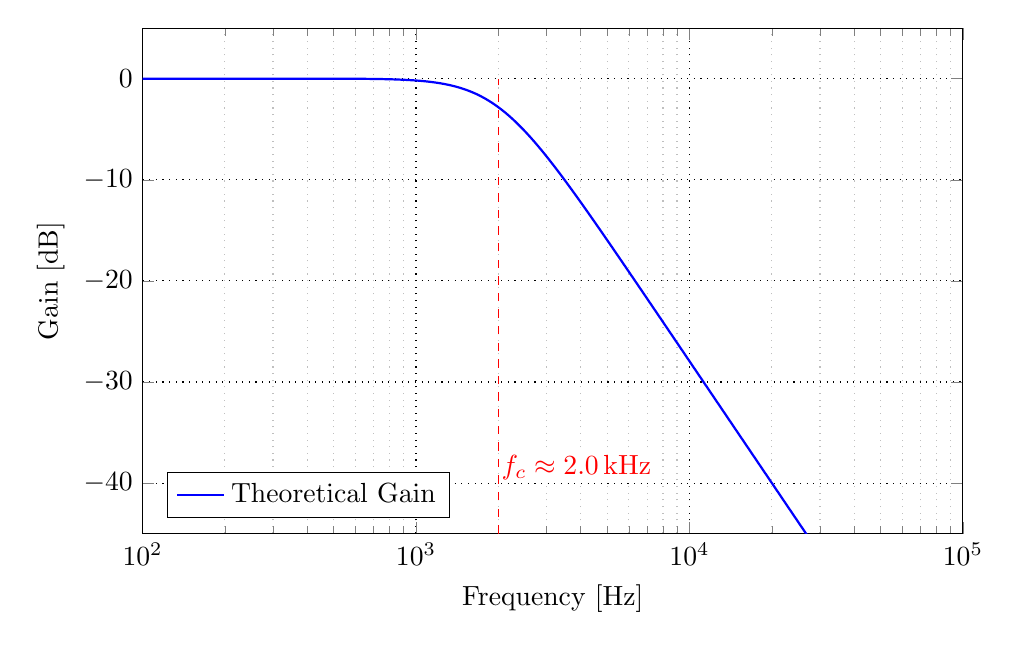
\begin{tikzpicture}
    \begin{semilogxaxis}[
        width=12cm, height=8cm,
        xlabel={Frequency [Hz]},
        ylabel={Gain [dB]},
        grid=both,
        major grid style={dotted,black},
        minor grid style={dotted,gray!50},
        xmin=100, xmax=100000,
        ymin=-45, ymax=5,
        domain=100:100000,
        samples=200,
        legend pos=south west,
      ]
      % Define constants: R=50e3, C1=2.3e-9, C2=1.1e-9
      % fc = 1/(2*pi*sqrt(R*R*C1*C2)) = 2001 Hz
      % Q = sqrt(C1/C2)/2 = sqrt(2.3/1.1)/2 = 0.723
      % Transfer function H(f) magnitude in dB:
      % 20*log10( 1 / sqrt( (1-(f/fc)^2)^2 + ( (f/fc)/Q )^2 ) )
      \addplot[thick, blue] {20*log10( 1 / sqrt( (1-(x/2001)^2)^2 + ( (x/2001)/0.723 )^2 ) ) };
      \addlegendentry{Theoretical Gain}
      
      % Mark Cutoff frequency
      \draw[dashed, red] (axis cs: 2001, -45) -- (axis cs: 2001, 0);
      \node[red, anchor=south west, fill=white, inner sep=1pt] at (axis cs: 2001, -40) {$f_c \approx \SI{2.0}{\kilo\hertz}$};
    \end{semilogxaxis}
  \end{tikzpicture}
  \caption{サレン・キー型LPFの理論周波数特性(ボード線図)}
  \label{fig:lpf_bode}
\end{figure}

% ===== 参考文献 =====
\begin{thebibliography}{99}
    \bibitem{kaneko1977_1} 金子尚志:「PCM 通信の技術」,産報出版株式会社,pp.17-19 (1977).
    \bibitem{hatori2012} 羽鳥光俊:「わかりやすい通信工学」,コロナ社,p.21 (2012).
    \bibitem{kaneko1977_2} 金子尚志:「PCM 通信の技術」,産報出版株式会社,p.27 (1977).
    \bibitem{takasaki2021} 高崎和之:「基本からわかる電子回路」,株式会社ナツメ社,pp.36-37 (2021).
    \bibitem{terashima2019} 寺島一彦,兼重明宏:「制御工学 技術者のための,理論・設計から実装まで」,実教出版株式会社,pp.121-128 (2019).
    \bibitem{kaneko1977_3} 金子尚志:「PCM 通信の技術」,産報出版株式会社,pp.14-15 (1977).
    \bibitem{kaneko1977_4} 金子尚志:「PCM 通信の技術」,産報出版株式会社,pp.10-11 (1977).
    \bibitem{kaneko1977_5} 金子尚志:「PCM 通信の技術」,産報出版株式会社,p.10 (1977).
    % --- 以下,Web参考文献 ---
    \bibitem{analog_quantization} Analog Devices: "MT-001: Taking the Mystery out of the Infamous Formula, SNR = 6.02N + 1.76dB, and Why You Should Care", \url{https://www.analog.com/media/en/training-seminars/tutorials/MT-001.pdf} (参照 2025-12-04).
    \bibitem{ti_sallen_key} Texas Instruments: "Analysis of the Sallen-Key Architecture (Rev. B)", \url{https://www.ti.com/lit/an/sloa024b/sloa024b.pdf} (参照 2025-12-04).
    % ローム株式会社 TechWeb:ADコンバータの動作原理,標本化と量子化に関する技術解説
    \bibitem{rohm_techweb} ローム株式会社:「TechWeb - ADコンバータの基礎」,\url{https://techweb.rohm.co.jp/product/conversion-logic-circuits/ad-converters/23878/} (参照 2025-12-04).
    % Engineer Climb:ADコンバータの変換原理とサンプリング・量子化の解説記事
    \bibitem{engineer_climb} Engineer Climb:「【ADコンバータ】変換原理とサンプリング・量子化を解説」,\url{https://engineer-climb.com/adc-basic/} (参照 2025-12-04).
\end{thebibliography}
\end{document}